\documentclass{article}

\usepackage[margin=1.0in]{geometry}
\usepackage{graphicx}
\usepackage{amsmath}
\usepackage{float}
\usepackage{enumitem}
\usepackage{gensymb}

\title{CSC 577 HW5}
\date{2/20/2019}
\author{Simon Swenson}

\begin{document}

\pagenumbering{gobble}
\maketitle
\pagenumbering{arabic}

\section{Introduction}

In this assignment, we solved for the camera matrix from our labeled points, 
used that camera matrix (and a light) to render a Lambertian sphere. We also 
attempted to decompose the camera matrix into its component parts. However, 
after spending some time substituting variables in the many equations by hand 
(18 equations with 15 unknowns), it became clear that I would run out of time 
before finishing this exercise. Thus, another approach was used: MATLAB's fsolve 
function. Even this method was unable to solve for the unknown parameters, 
though. At the very least, we have the camera matrix written symbolically in 
terms of the variables that we want to know.

\section{Camera Matrix}

Solving for the camera matrix was fairly straightforward, since we had labeled 
data. I used the eigenvector 
method for finding the homogeneous linear least squared solution, doubling the 
number of rows in the $U$ matrix and structuring it as we derived in class. The 
solution is below:

$$
M = \begin{bmatrix}
 0.0308 & 0.0520 & -0.1349 & 0.4846 \\
-0.1387 & 0.0480 & -0.0248 & 0.8492 \\
 0      & 0      &  0      & 0.0009
\end{bmatrix}
$$

\subsection{Visualization}

Given this matrix, we can visually compare world coordinates sent through the 
camera matrix into pixel coordinates to the ground truth:

\begin{figure}[!ht]
	\centering
	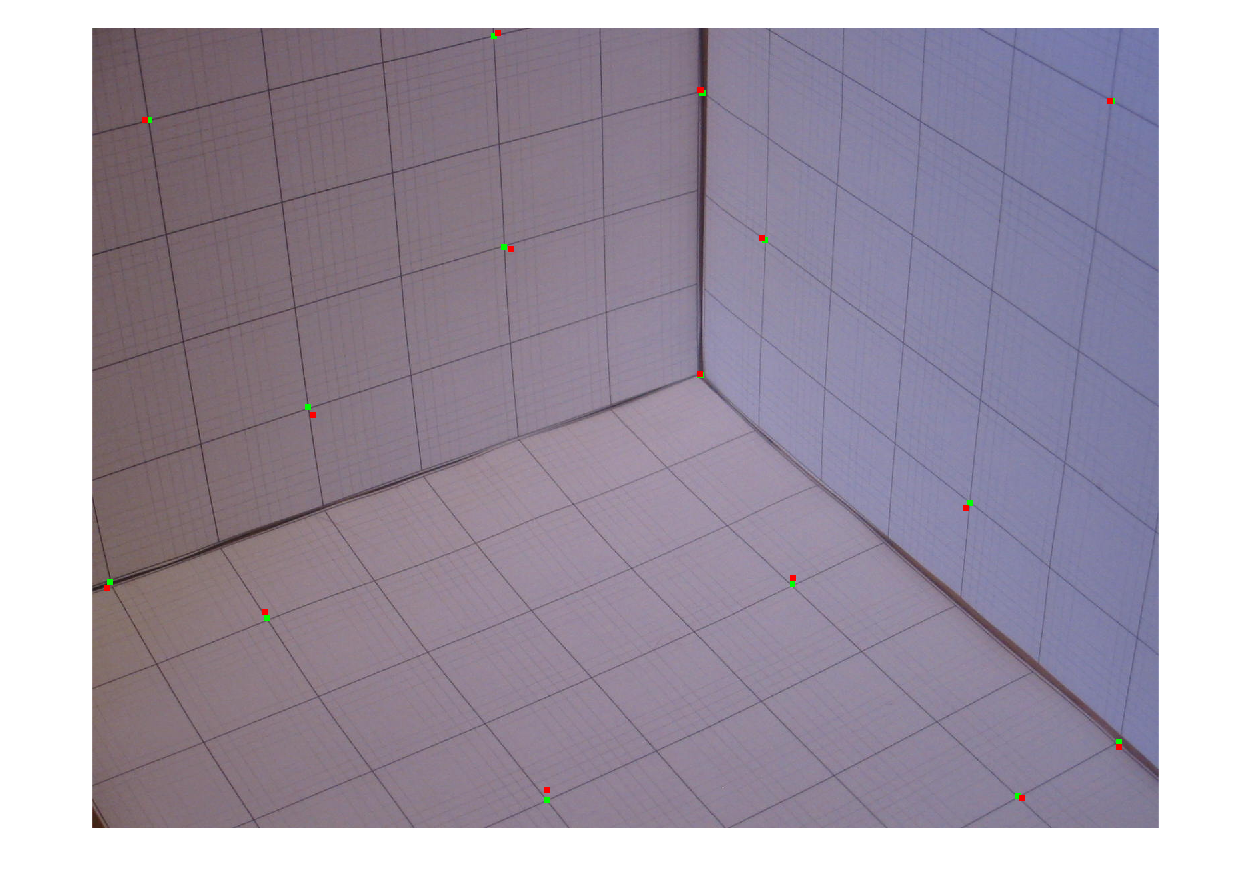
\includegraphics[width=120mm]{figs/ground_truth_to_hlse_sln.png}
	\caption{A comparison between world coordinates sent through the camera 
        matrix to pixel coordinates and the ground truth. Ground truth is in 
        green, projected points are in red. The matrix is not perfect, and 
        certainly appears to get worse near the edges of the screen, but it 
        looks better than the two other camera matrices from the last 
        assignment.}
\end{figure}

\subsection{Error Comparison}

The points definitely visually look closer than the matrices from the last 
assignment, but is that actually the case? After computing the RMSE between 
ground truth and projected points, we can compare it to the 
RMSE of the matrices from the previous assignment:

\begin{tabular}{r | r}
    Proposed Matrix \#1 (from HW4) &         20.9578 \\
    Proposed Matrix \#2 (from HW4) &         52.1719 \\
                     Solved Matrix & \enspace 8.5947
\end{tabular}

As can be seen from the table above, our solution is \textit{much} better than 
the other two proposed camera matrices. Is this expected? Recall the original 
formulation of a homogeneous line:

$$
a x + b y = d
$$
$$
a^2 + b^2 = 1
$$
 
And the corresponding error metric used in the homogeneous least squares problem:

$$
E = \sum (d - a x_i - b y_i)^2
$$

Recall that, in class, we defined $d_i$ to be the perpendicular distance between 
an arbitrary point in the space and the line. We also derived the following equation: 

\begin{align}
d + d_i &= x_i * \hat{n} \\
d_i &= x_i * \hat{n} - d
\end{align}

After realizing that the normal vector is just $(a, b)$, the sum of the squares 
of $d_i$ is our error metric. This (squared) formulation is monotonic with the 
perpendicular distance, so it is a valid error metric. And, now compare it to 
the definition of the RMSE metric:

\begin{align}
RMSE &= \sqrt{\frac{\sum_i distance(y_i, M x_i)^2}{N}} \\
RMSE &\propto \frac{\sum_i distance(y_i, M x_i)^2}{N} \\
RMSE &\propto \sum_i distance(y_i, M x_i)^2
\end{align}

Note that distance in the above equation is the cartesian distance, which is 
exactly the same as the perpendicular distance between the line and the point 
in the original error metric. $N$ is basically a constant, and the square root 
can be multiplied out, so we end up with the sum of the squared distance in 
the second equation, which is essentially our error metric from above. Thus, 
RMSE a perfect error metric to report, since it is what our solution minimized. 
This behavior is good, as it minimizes the sum of the distance between each 
point and the line. However, there might be better error metrics, but sum of 
squared distances is easy to understand and straightforward to implement a 
solution for.

\section{Rendering a Sphere}

If we add a light to the scene, we can start rendering objects using the 
Lambertian shading model. If the light is at a known location, recall that, all 
we need to know to shade a fragment of an object is that fragment's location in world space (to determine 
the vector from light to surface) and normal. Additionally, to cull 
back faces, we need to know the camera's facing, as well (which can be derived 
from the camera matrix).

To shade a pure white sphere, we iterate over points in the sphere. We find the 
distance between the light and sphere fragment to be shaded, then we normalize 
that vector (we say that the light intensity is 1). The normal of the sphere 
fragment is easy to find, since we know the center of the sphere. We just find 
the distance between the sphere fragment and the center of the sphere and 
normalize that. At this point, we can determine whether the fragment faces the 
camera or not. If its norm dotted with the distance between the fragment and the 
camera is positive, the fragment points away, and we can move on to the next 
fragment. If not, we dot the two vectors and multiply by the albedo. I used 
an albedo of 255 (pure white). We ensure pixel values are not negative by 
choosing the max between the pixel value and 0.

\begin{figure}[!ht]
	\centering
	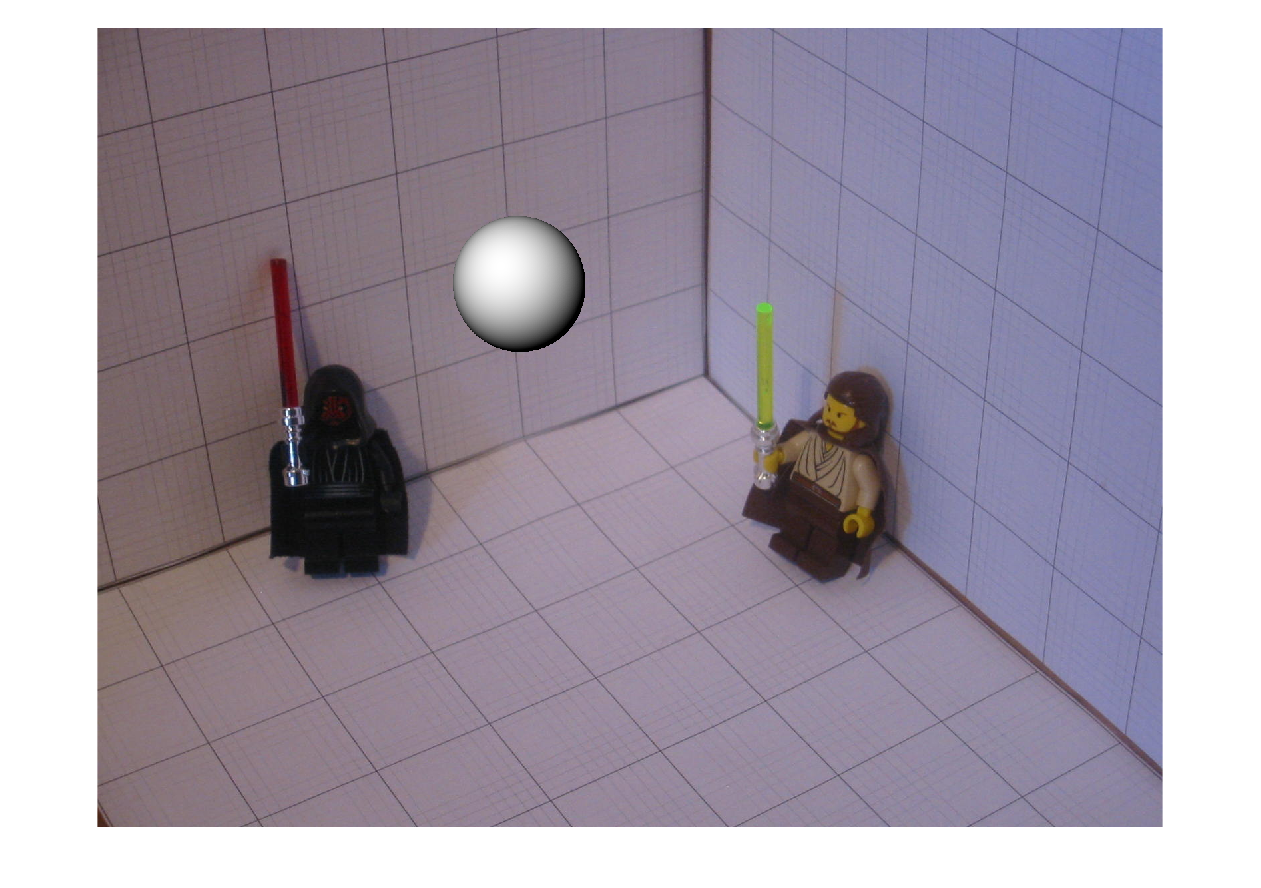
\includegraphics[width=120mm]{figs/sphere.png}
	\caption{A sphere rendered at (3, 2, 3) with radius 0.5. The light is 
        assumed to come from (33, 29, 44), and the camera is assumed to be at 
        (9, 14, 11).}
\end{figure}

To me, this sphere looks a little off-centered (to the left of where it should 
be), so I rendered some dots at that same z coordinate from 0 to 5 to 
double-check. Sure enough, the sphere is roughly in the correct spot. As z 
increases, the positions move further to the left, and I was comparing the 
sphere's location to the position (3, 2, 0) on the graph paper.

\begin{figure}[!ht]
	\centering
	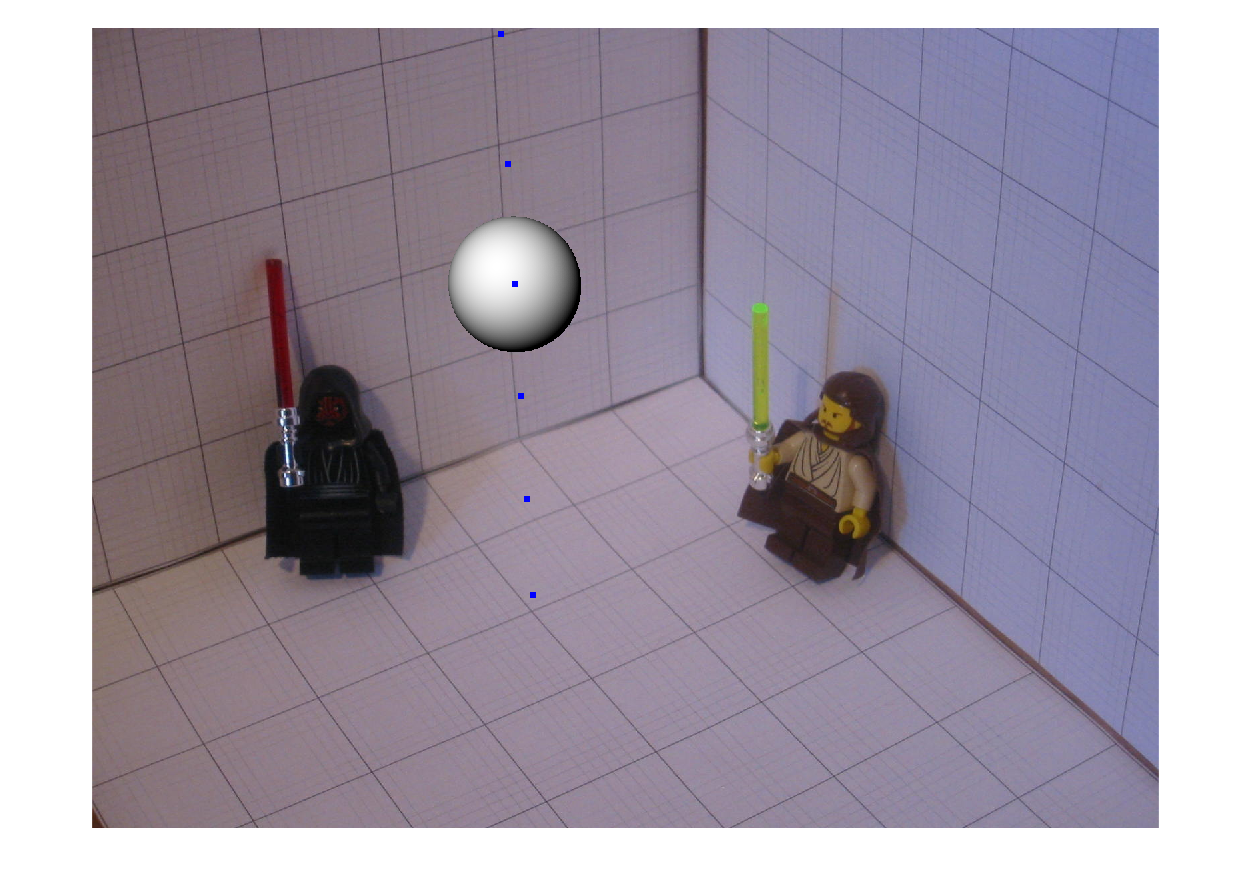
\includegraphics[width=120mm]{figs/sphere_dbl_check.png}
	\caption{Double-checking the sphere. Now that the dots are added, the sphere 
        doesn't appear to be too far to the left, anymore. It was an optical 
        illusion.}
\end{figure}

\section{Decomposing the Camera Matrix}

In theory, it should be possible to decompose the camera matrix into its 
component parts. If we assume the MATLAB coordinate system, we have the following 
intrinsic matrices:

$$
I_t = 
\begin{bmatrix}
1 & 0 & \frac{h}{2} \\
0 & 1 & \frac{w}{2} \\
0 & 0 & 1
\end{bmatrix}
$$
$$
I_{rf} = 
\begin{bmatrix}
0 & -1 &  0 \\
1 &  0 &  0 \\
0 &  0 & -1
\end{bmatrix}
$$
$$
I_s = 
\begin{bmatrix}
\frac{h}{2} &           0 & 0 \\
0           & \frac{h}{2} & 0 \\
0           &           0 & 1
\end{bmatrix}
$$

Coming from the last assignment, most of these should come as no surprise. These 
are essentially the matrices used to derive a mapping between standard image 
coordinates to pixel coordinates (and vise versa).
However, there is one small monkey-wrench that must be dealt with. The camera 
coordinate system is right-handed. This means that the last axis points away 
from the scene rather than towards it. This means that points that we want to 
render will get sent to -w values. In standard image coordinates, we wanted to 
map (1, 1, 1) to (0, 1400). However, if we perform the same transformation on 
the point (1, 1, -1), we'll end up at (1200, 200), essentially flipping both 
axes. We can easily fix this by negating w in the rotation/flip matrix, hence 
the last entry of -1 instead of 1.

Multiplying these matrices out, we have:

\begin{align}
I &= I_t I_{rf} I_s \\
  &= \begin{bmatrix}
1 & 0 & \frac{h}{2} \\
0 & 1 & \frac{w}{2} \\
0 & 0 & 1
\end{bmatrix} \begin{bmatrix}
0 & -1 &  0 \\
1 &  0 &  0 \\
0 &  0 & -1
\end{bmatrix}\begin{bmatrix}
\frac{h}{2} &           0 & 0 \\
0           & \frac{h}{2} & 0 \\
0           &           0 & 1
\end{bmatrix} \\
  &= \begin{bmatrix}
1 & 0 & \frac{h}{2} \\
0 & 1 & \frac{w}{2} \\
0 & 0 & 1
\end{bmatrix} \begin{bmatrix}
0           & -\frac{h}{2} &  0 \\
\frac{h}{2} &            0 &  0 \\
0           &            0 & -1
\end{bmatrix} \\
  &= \begin{bmatrix}
0           & -\frac{h}{2} &  -\frac{h}{2} \\
\frac{h}{2} &            0 &  -\frac{w}{2} \\
0           &            0 &            -1
\end{bmatrix}
\end{align}

Second, we have the projection matrix, which is easy:

$$
P = \begin{bmatrix}
1 & 0 & 0 & 0 \\
0 & 1 & 0 & 0 \\
0 & 0 & 1 & 0
\end{bmatrix}
$$

Lastly, we have the extrinsic matrices, which can be represented as a 
translation followed by a rotation. If we want to solve for the camera's 
location in terms of the translation, we just negate the translation terms. For 
the rotation matrix, we need to be a bit careful. We have some restrictions on 
the new basis vectors, call them $f, g, h$. We want each vector to be 
normal. We also want them to be orthogonal. Finally, we want the cross product 
of the first two to equal the third. This handles both h being normal and the 
basis being right-handed. Let's handle these equations first:

$$
f_1^2 + f_2^2 + f_3^2 = 1
$$
$$
g_1^2 + g_2^2 + g_3^2 = 1
$$
$$
f_1 g_1 + f_2 g_2 + f_3 g_3 = 0
$$
\begin{align}
h &= f \times g \\
\begin{bmatrix}
h_1 \\
h_2 \\
h_3
\end{bmatrix} &= \begin{vmatrix}
i & j & k \\
f_1 & f_2 & f_3 \\
g_1 & g_2 & g_3
\end{vmatrix} \\
&= \begin{bmatrix}
f_2 g_3 - f_3 g_2 \\
f_1 g_3 - f_3 g_1 \\
f_1 g_2 - f_2 g_1
\end{bmatrix}
\end{align}

Since these equations aren't involved in the main camera matrix, directly, let's 
ignore them for now (until we need them later to solve the system of equations). 
Let's now define the rotation and translation matrices. $(x, y, z)$ is the 
camera's position in 3-d space.

$$
E_r = \begin{bmatrix}
f_1 & f_2 & f_3 & 0 \\
g_1 & g_2 & g_3 & 0 \\
h_1 & h_2 & h_3 & 0 \\
  0 &   0 &   0 & 1 \\
\end{bmatrix}
$$
$$
E_t = \begin{bmatrix}
1 & 0 & 0 & -x \\
0 & 1 & 0 & -y \\
0 & 0 & 1 & -z \\
0 & 0 & 0 &  1 \\
\end{bmatrix}
$$

So, the entire extrinsic matrix is:

\begin{align}
E &= E_r E_t \\
  &= \begin{bmatrix}
f_1 & f_2 & f_3 & 0 \\
g_1 & g_2 & g_3 & 0 \\
h_1 & h_2 & h_3 & 0 \\
  0 &   0 &   0 & 1 \\
\end{bmatrix} \begin{bmatrix}
1 & 0 & 0 & -x \\
0 & 1 & 0 & -y \\
0 & 0 & 1 & -z \\
0 & 0 & 0 &  1 \\
\end{bmatrix} \\
  &= \begin{bmatrix}
f_1 & f_2 & f_3 & -(f_1 x + f_2 y + f_3 z) \\
g_1 & g_2 & g_3 & -(g_1 x + g_2 y + g_3 z) \\
h_1 & h_2 & h_3 & -(h_1 x + h_2 y + h_3 z) \\
  0 &   0 &   0 &                        1
\end{bmatrix}
\end{align}

Combining the three matrices, we have:

\begin{align}
C &= I P E \\
  &= \begin{bmatrix}
0           & -\frac{h}{2} &  -\frac{h}{2} \\
\frac{h}{2} &            0 &  -\frac{w}{2} \\
0           &            0 &            -1
\end{bmatrix} \begin{bmatrix}
1 & 0 & 0 & 0 \\
0 & 1 & 0 & 0 \\
0 & 0 & 1 & 0
\end{bmatrix} \begin{bmatrix}
f_1 & f_2 & f_3 & -(f_1 x + f_2 y + f_3 z) \\
g_1 & g_2 & g_3 & -(g_1 x + g_2 y + g_3 z) \\
h_1 & h_2 & h_3 & -(h_1 x + h_2 y + h_3 z) \\
  0 &   0 &   0 &                        1
\end{bmatrix} \\
  &= \begin{bmatrix}
0           & -\frac{h}{2} &  -\frac{h}{2} \\
\frac{h}{2} &            0 &  -\frac{w}{2} \\
0           &            0 &            -1
\end{bmatrix} \begin{bmatrix}
f_1 & f_2 & f_3 & -(f_1 x + f_2 y + f_3 z) \\
g_1 & g_2 & g_3 & -(g_1 x + g_2 y + g_3 z) \\
h_1 & h_2 & h_3 & -(h_1 x + h_2 y + h_3 z)
\end{bmatrix} \\
  &= \begin{bmatrix}
-\frac{h}{2}(g_1 + h_1) & -\frac{h}{2}(g_2 + h_2) & -\frac{h}{2}(g_3 + h_3) & \frac{h}{2}(x(g_1 + h_1) + y(g_2 + h_2) + z(g_3 + h_3)) \\
\frac{1}{2}(h f_1 - w h_1) & \frac{1}{2}(h f_2 - w h_2) & \frac{1}{2}(h f_3 - w h_3) & \frac{1}{2}(w(h_1 x + h_2 y + h_3 z) - h(f_1 x + f_2 y + f_3 z)) \\
                   -h_1 &                    -h_2 &                    -h_3 & h_1 x + h_2 y + h_3 z
\end{bmatrix}
\end{align}

Since we know the camera matrix (with norm 1), we can represent this new symbolic 
matrix in terms of the old matrix's values times $\rho$:

$$
\rho M = C
$$

This essentially gives us 12 equations to work with (one for each matrix index). 
However, we have 15 
unknowns. Thus, when we incorporate the constraints on the dot products and 
cross products, we have 18 equations with 15 unknowns, which is doable.

(I realized after the fact by reviewing the slides that rotation is often 
represented as three angles rather than three orthogonal unit vectors. I will 
redo the above steps with angles if I have time.)

From here, it's a plug and chug. Solve for one unknown, substitute into the 
remaining equations, and so on, until a solution for a single unknown is 
reached. Then propagate the results back. Doing this by hand is very tedeous (at 
least with the above derivation), though, and I unfortunately ran out of time to 
do so, after solving about six of the unknowns in terms of the other variables. 
The equations were starting to take up a lot of space on the page. 

Anyway, this is no excuse, so I tried to solve this problem another way: by 
by using a symbolic math library. Luckily, MATLAB actually has a function for 
solving systems of non-linear equations, fsolve. I programmed things into 
MATLAB and asked it to solve, but fsolve kept giving warnings such as:

\begin{quote}
fsolve stopped because the problem appears regular as measured by the gradient,
but the vector of function values is not near zero as measured by the
default value of the function tolerance.
\end{quote}

It appears that the algorithm that MATLAB was using reached a stopping point 
(based on the gradient), but not all of the equations are satisfied. You can 
take a look at the MATLAB code, if you'd like, but, for me, it's back to the 
drawing board!

\end{document}